\documentclass[dvipsnames]{standalone}
\usepackage{pgfplots}
\usepgfplotslibrary{ternary}
\usetikzlibrary{shapes}
\begin{document}
\definecolor{purple}{HTML}{520066}
\definecolor{blue}{HTML}{31688e}
\definecolor{green}{HTML}{35b779}
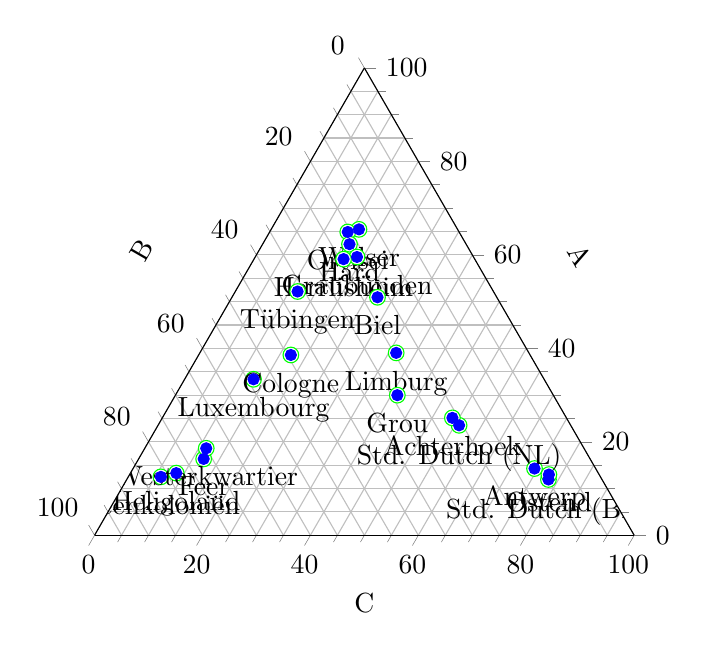
\begin{tikzpicture}
	\tikzstyle{ingv}=[circle, green, draw, inner sep = 2pt, fill=white]
	\tikzstyle{dutch}=[ingv, fill=green]
	\tikzstyle{central}=[ingv, rectangle, blue, fill=blue]
	\tikzstyle{upper}=[ingv, regular polygon, regular polygon sides=3, purple, fill=purple, inner sep = 1pt]
	\begin{ternaryaxis}[
		xmin = 0, xmax = 1,
		ymin = 0, ymax = 1,
		zmin = 0, zmax = 1,
		xlabel = A, ylabel = B, zlabel = C,
		grid = both, label style = {sloped},
		minor tick num = 3,
	]
	\addplot3[only marks, mark options={blue}] table {
		0.6546	0.1827	0.1627
		0.649	0.2063	0.1447
		0.6229	0.2161	0.161
		0.5955	0.2159	0.1886
		0.5909	0.2431	0.166
		0.5216	0.3628	0.1155
		0.5093	0.221	0.2697
		0.3903	0.2459	0.3638
		0.125	0.8146	0.0605
		0.133	0.7821	0.0849
		0.1634	0.7161	0.1205
		0.1861	0.7	0.1139
		0.3338	0.5385	0.1277
		0.3858	0.4433	0.1709
		0.1194	0.0992	0.7814
		0.1299	0.0931	0.777
		0.1428	0.1133	0.7439
		0.2353	0.2068	0.5579
		0.2512	0.2113	0.5375
		0.2998	0.289	0.4112
	};
	\node[ingv, label=below:Walser] at (axis cs:0.6546, 0.1827, 0.1627) {};
	\node[ingv, label=below:Ortisei] at (axis cs:0.649, 0.2063, 0.1447) {};
	\node[ingv, label=below:Hard] at (axis cs:0.6229, 0.2161, 0.161) {};
	\node[ingv, label=below:Graub\"{u}nden] at (axis cs:0.5955, 0.2159, 0.1886) {};
	\node[ingv, label=below:Herrlisheim] at (axis cs:0.5909, 0.2431, 0.166) {};
	\node[ingv, label=below:T\"{u}bingen] at (axis cs:0.5216, 0.3628, 0.1155) {};
	\node[ingv, label=below:Biel] at (axis cs:0.5093, 0.221, 0.2697) {};
	\node[ingv, label=below:Limburg] at (axis cs:0.3903, 0.2459, 0.3638) {};
	\node[ingv, label=below:Veenkoloni\"{e}n] at (axis cs:0.125, 0.8146, 0.0605) {};
	\node[ingv, label=below:Heligoland] at (axis cs:0.133, 0.7821, 0.0849) {};
	\node[ingv, label=below:Feer] at (axis cs:0.1634, 0.7161, 0.1205) {};
	\node[ingv, label=below:Westerkwartier] at (axis cs:0.1861, 0.7, 0.1139) {};
	\node[ingv, label=below:Luxembourg] at (axis cs:0.3338, 0.5385, 0.1277) {};
	\node[ingv, label=below:Cologne] at (axis cs:0.3858, 0.4433, 0.1709) {};
	\node[ingv, label=below:Std. Dutch (BE)] at (axis cs:0.1194, 0.0992, 0.7814) {};
	\node[ingv, label=below:Ostend] at (axis cs:0.1299, 0.0931, 0.777) {};
	\node[ingv, label=below:Antwerp] at (axis cs:0.1428, 0.1133, 0.7439) {};
	\node[ingv, label=below:Std. Dutch (NL)] at (axis cs:0.2353, 0.2068, 0.5579) {};
	\node[ingv, label=below:Achterhoek] at (axis cs:0.2512, 0.2113, 0.5375) {};
	\node[ingv, label=below:Grou] at (axis cs:0.2998, 0.289, 0.4112) {};
	\end{ternaryaxis}
\end{tikzpicture}
\end{document}